\documentclass[11pt,a4paper]{article}
\usepackage[T1]{fontenc}
\usepackage{lmodern}
\usepackage[margin=2.2cm]{geometry}
\usepackage{amsmath,amssymb}
\usepackage{booktabs,tabularx,array}
\usepackage{graphicx}
\usepackage{float}
\usepackage{longtable}
\usepackage{xcolor}
\usepackage{tikz}
\usetikzlibrary{arrows.meta,positioning}
\usepackage[hidelinks]{hyperref}
\def\sectionautorefname{Section}\def\subsectionautorefname{Section}

\definecolor{navy}{HTML}{1F3A5F}
\definecolor{soft}{HTML}{EEF3FA}
\definecolor{todo}{HTML}{FDF1E9}
\definecolor{todoline}{HTML}{EB6834}
\definecolor{warnbg}{HTML}{FCEBEB}
\newcommand{\code}[1]{\texttt{\small #1}}
% A box the author fills in: the course does not allow LLM-written analysis or conclusions.
\newcommand{\authorbox}[2]{\par\smallskip\noindent\fcolorbox{todoline}{todo}{\parbox{\dimexpr\linewidth-2\fboxsep-2\fboxrule}{%
  \small\textbf{To be written by the author --- #1}\par\smallskip #2}}\par\smallskip}

% generated by make_figures.py
\newcommand{\ensfive}{0.797}
\newcommand{\ensthree}{0.793}
\newcommand{\foneEeight}{0.776}
\newcommand{\foneEfive}{0.600}
\newcommand{\foneEfour}{0.661}
\newcommand{\foneEone}{0.770}
\newcommand{\foneEseven}{0.773}
\newcommand{\foneEsix}{0.785}
\newcommand{\foneEthree}{0.754}
\newcommand{\foneEtwo}{0.753}
\newcommand{\foneablfirst}{0.754}
\newcommand{\foneablfirstlast}{0.778}
\newcommand{\foneablspread}{0.778}
\newcommand{\kdinfer}{6}
\newcommand{\kdparams}{62.8M}
\newcommand{\kdretain}{98.8}
\newcommand{\medtest}{3,932}
\newcommand{\medtrain}{2,469}
\newcommand{\medval}{3,771}
\newcommand{\ndev}{3,505}
\newcommand{\nfn}{250}
\newcommand{\nfp}{176}
\newcommand{\ntest}{1,517}
\newcommand{\ntestindev}{1,517}
\newcommand{\ntrain}{31,677}
\newcommand{\ntraindup}{5,710}
\newcommand{\ntrainraw}{37,387}
\newcommand{\ntrainuniq}{31,677}
\newcommand{\nval}{1,988}
\newcommand{\nzips}{16}
\newcommand{\shortereight}{55}
\newcommand{\teacherinfer}{20}
\newcommand{\teacherparams}{88.0M}
\newcommand{\testhaslabel}{yes}
\newcommand{\trainzero}{58.6}

\makeatletter\newcommand{\tabinput}[1]{\@@input #1 }\makeatother % expandable \input inside tabulars

\title{\textbf{CS-781 Capstone, Phase 4: Court Judgment Prediction}\\[2pt]
\large A hierarchical chunk classifier on the four Phase-1 language models}
\author{Manish Kumar (251330604)\\ CS-781, IIT Kanpur}
\date{October 2026}

\begin{document}
\maketitle

\begin{abstract}
\noindent We predict the binary outcome of Indian court judgments from their text, starting from the four
legal language models pre-trained in Phase~1.  A judgment is cut into 512-token chunks; eight chunks are
encoded by the Phase-1 backbone, mean-pooled, read by a BiGRU with attention pooling and classified.
Eight experiments cover all four architectures and seven adaptation techniques (full and partial
fine-tuning, gradual unfreezing, BitFit, LoRMA+, AdaLoRA and Houlsby adapters) plus knowledge distillation.
Because every test document also appears, labelled, in the provided development file, all model selection uses
only the \nval{} development documents that are not in the test set.  On that clean validation set the best
single model (A4, top four blocks fine-tuned) reaches macro-F1 \foneEsix, the distilled 6-block student
\foneEeight{} (\kdretain\% of its teacher with \kdparams{} instead of \teacherparams{} parameters), and an
average of five models \ensfive.  Reading the last chunks of a judgment scores higher than reading the first
(\foneEsix{} vs \foneablfirst).  All numbers are generated from the run outputs by
\code{p4/report/make\_figures.py}.
\end{abstract}

\tableofcontents
\newpage

% =====================================================================
\section{Introduction}
Court judgment prediction (CJPE) asks for the outcome of a case (label 1: the appeal is allowed or the order
set aside; label 0: dismissed) from the judgment text, with the final decision removed; the data follow the ILDC corpus \cite{malik2021ildc} (single- and
multi-instance training sets combined).  The primary metric is
macro-F1 over the two classes, with precision and recall as secondary metrics.  Judgments are long (median
\medtrain{} BPE tokens in training, \medval{} in validation), so the model must represent a long document.
The rules require the Phase-1 models as the only pretrained weights, all four architectures across the
submissions, at least six substantially different experiments with at least five adaptation techniques, LoRMA
and knowledge distillation.

% =====================================================================
\section{Data and integrity checks}\label{sec:data}
\begin{table}[H]\centering\small
\caption{Splits used (lengths in Phase-1 BPE tokens).}\label{tab:data}
\begin{tabular}{lrrrrr}\toprule
Split & Documents & Label 0 / 1 & Median length & 90th pct. & Tokens\\\midrule
\tabinput{tables/data.tex}
\bottomrule\end{tabular}\end{table}

\paragraph{Findings in the provided files.} Three checks were made before any training
(\code{p4/cj/data.py}):
\begin{itemize}
  \item \texttt{test.json} carries a \code{label} field for every test document (\testhaslabel).  It is dropped
  when the file is loaded and never read.
  \item All \ntestindev{} of the \ntest{} test documents occur verbatim, with their labels, in \texttt{dev.json}
  (\ndev{} documents).  Selecting models or thresholds on the full development file would therefore tune on the
  test answers.  We use as validation only the \nval{} development documents whose text is not in the test set
  (994 / 994 labels).
  \item The training file has \ntrainraw{} entries but only \ntrainuniq{} distinct texts (\ntraindup{} exact
  duplicates, none with conflicting labels).  Duplicates are removed.
\end{itemize}
Training is \trainzero\% label 0, while validation (and the test set, by its size) is balanced.

\begin{figure}[H]\centering
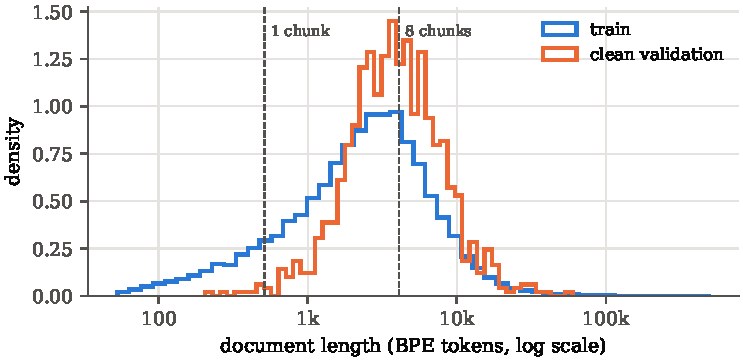
\includegraphics[width=0.8\linewidth]{figs/lengths.pdf}
\caption{Document lengths. Eight 512-token chunks cover the whole document for \shortereight\% of the
validation documents.}
\label{fig:lengths}\end{figure}

% =====================================================================
\section{Methods}
\subsection{Hierarchical chunk model}
\begin{figure}[H]\centering
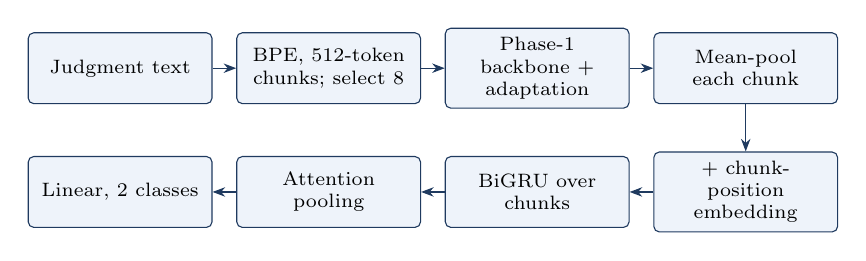
\begin{tikzpicture}[node distance=3mm, box/.style={draw=navy,rounded corners=2pt,fill=soft,align=center,
  font=\scriptsize,minimum height=9mm,text width=21mm}, arr/.style={-{Stealth[length=1.6mm]},navy}]
  \node[box] (a) {Judgment text};
  \node[box,right=of a] (b) {BPE, 512-token chunks; select 8};
  \node[box,right=of b] (c) {Phase-1 backbone + adaptation};
  \node[box,right=of c] (d) {Mean-pool each chunk};
  \node[box,below=6mm of d] (e) {+ chunk-position embedding};
  \node[box,left=of e] (f) {BiGRU over chunks};
  \node[box,left=of f] (g) {Attention pooling};
  \node[box,left=of g] (h) {Linear, 2 classes};
  \foreach \x/\y in {a/b,b/c,c/d,d/e,e/f,f/g,g/h} \draw[arr] (\x)--(\y);
\end{tikzpicture}
\caption{The CJPE model (\code{p4/cj/model.py}).}
\label{fig:model}\end{figure}

\begin{itemize}
  \item \textbf{Chunking} (\code{data.strategy}). The document is tokenized once and cut into chunks of 512
  tokens; eight are kept: the \emph{last} eight (default; aligned to the end of the document), the \emph{first}
  eight, \emph{first four + last four}, or eight \emph{spread} evenly.  Shorter documents use all their chunks.
  \item \textbf{Chunk vector}: the mean of the backbone's final hidden states over the chunk's tokens.
  \item \textbf{Document layer}: projection to 256 dimensions plus a learned chunk-position embedding, a
  one-layer BiGRU \cite{cho2014gru} over the chunk sequence and attention pooling with a learned scoring vector
  (hierarchical attention, \cite{yang2016han}); a linear layer gives two logits.
  \item \textbf{Backbones}: A1 and A4 keep their Phase-1 causal mask (best in Phase~3), A3 reads each chunk as its
  bidirectional prefix, A2 uses its decoder states (its encoder output is nearly collapsed, Phase-2 report).
  All use the cleaned 1B-token Phase-1 checkpoints.
\end{itemize}

\subsection{Adaptation techniques}
\begin{itemize}
  \item \textbf{Full fine-tuning} (E1): every weight.
  \item \textbf{Partial / layer-wise fine-tuning} (E6): the top four of A4's ten blocks and the final norm.
  \item \textbf{Layer freezing / unfreezing} (E7): ULMFiT-style gradual unfreezing \cite{howard2018ulmfit}; only
  the top block (and final norm) is trainable at the start, one more block is unfrozen every 300 optimizer
  steps, top to bottom, until the whole network trains.
  \item \textbf{BitFit} (E4) \cite{benzaken2022bitfit}: biases and norm gains only.
  \item \textbf{LoRMA+} (E2) \cite{bihany2025lorma}: $W=(I+\frac{\alpha}{r}BA)W_0$, $r=16$, $\alpha=32$, on the
  attention and MLP projections.
  \item \textbf{AdaLoRA} (E5) \cite{zhang2023adalora}: SVD-form update with importance-based rank pruning from 12
  to an average of 8 per module (implementation of Phase~3).
  \item \textbf{Houlsby adapters} (E3) \cite{houlsby2019adapters}: bottleneck 64 after attention and MLP.
  \item \textbf{Knowledge distillation} (E8) \cite{hinton2015kd}: the teacher is E6 (best single model); its
  logits on all \ntrain{} training documents are computed once (\code{dump\_logits.py}).  The student is A4 with
  6 of its 10 blocks (0, 2, 4, 5, 6, 8, keeping all three global-attention layers), fully fine-tuned with
  $0.5\,\mathrm{CE} + 0.5\,T^2\,\mathrm{KL}(p^T_\text{teacher}\,\|\,p^T_\text{student})$, $T=2$.
\end{itemize}

\subsection{Training and selection}\label{sec:train}
AdamW, 2 epochs over the \ntrain{} training documents (3{,}960 optimizer steps of 16 documents, 4 per
micro-batch), 6\% warm-up then cosine decay, weight decay 0.01, gradient clipping 1.0, bf16.  Learning rate
$5\times10^{-5}$ for full fine-tuning, gradual unfreezing and the KD student, $10^{-4}$ for partial
fine-tuning, $2\times10^{-4}$ for LoRMA+, adapters and AdaLoRA, and $10^{-3}$ for BitFit and the document
layer.  The PEFT runs were first started at $10^{-3}$ (the Phase-2/3 value); LoRMA+ and adapters stalled at a
training loss of 0.69 (chance) within the first 1{,}000 steps and were restarted at $2\times10^{-4}$, which is
the run reported here.  The loss is class-weighted cross-entropy (weights inverse to the training label
frequencies).  Every 250 steps the clean validation set is scored; the state with the best macro-F1 at the
validation-tuned decision threshold (grid 0.05--0.95) is kept, and that threshold is applied to the test set.

\subsection{Submissions}
\code{make\_submission.py} writes \code{prediction.json}, a list of \code{\{"id", "pred"\}} with one integer
0/1 for every test id in order, at the root of a zip.  Ensembles average the class-1 probabilities of several
runs and tune one threshold on their averaged validation probabilities.

% =====================================================================
\section{Results}
\subsection{All experiments}
\begin{table}[H]\centering
\caption{Clean-validation results (\nval{} documents). F1 = macro-F1 at the validation-tuned threshold
``thr''; F1@0.5 at the default threshold; P / R = macro precision / recall at thr.  Below the line: section
ablation of E6.}\label{tab:results}
\resizebox{\linewidth}{!}{\begin{tabular}{lllllrrrrrr}\toprule
Run & Arch & Method & Chunks & Trainable & \% & F1 & F1@0.5 & thr & P & R\\\midrule
\tabinput{tables/results.tex}
\bottomrule\end{tabular}}\end{table}

\begin{figure}[H]\centering
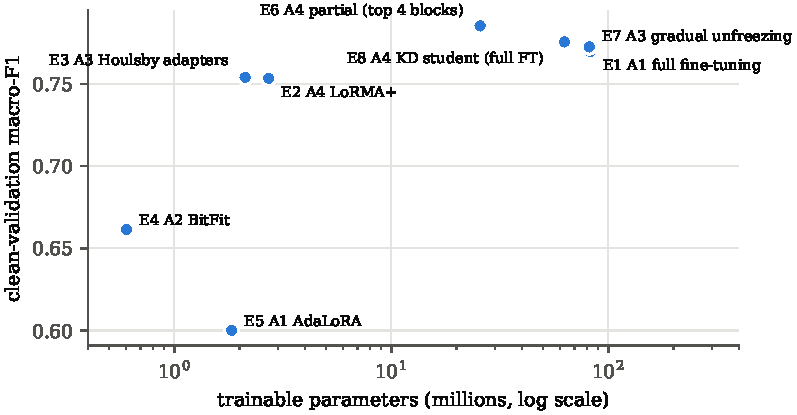
\includegraphics[width=0.85\linewidth]{figs/f1_vs_params.pdf}
\caption{Validation macro-F1 against the number of trained parameters (document layer included).}
\label{fig:params}\end{figure}

\begin{figure}[H]\centering
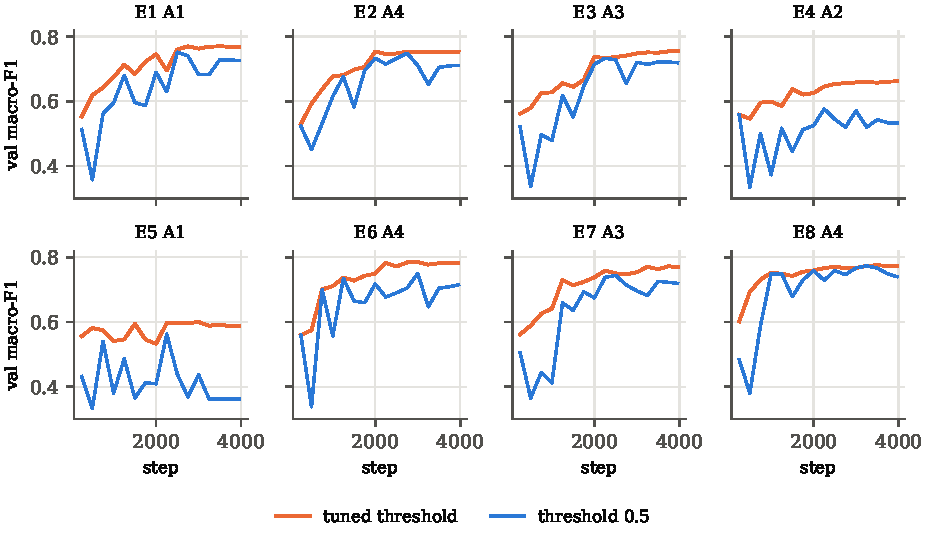
\includegraphics[width=0.95\linewidth]{figs/curves.pdf}
\caption{Validation macro-F1 during training, at the default and at the tuned threshold.}
\label{fig:curves}\end{figure}

\subsection{Decision threshold and class imbalance}
\begin{figure}[H]\centering
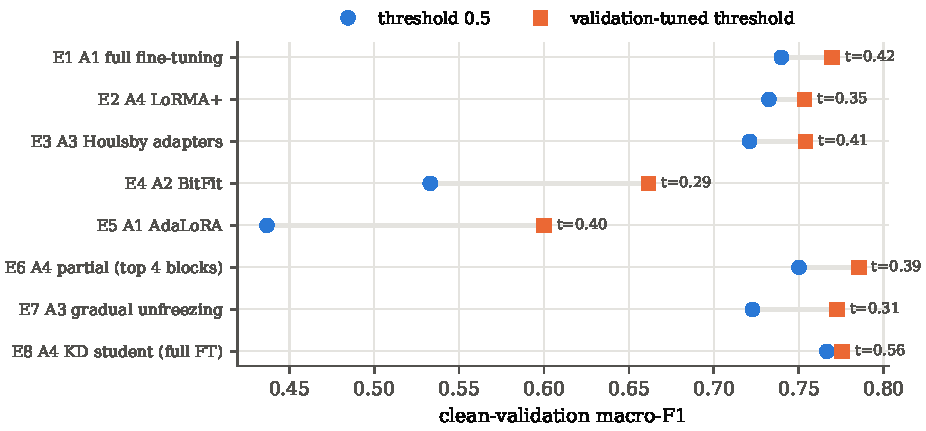
\includegraphics[width=0.85\linewidth]{figs/threshold.pdf}
\caption{Macro-F1 at threshold 0.5 and at the validation-tuned threshold $t$ (training is \trainzero\% label 0,
validation 50\%).}
\label{fig:thr}\end{figure}

\subsection{Which part of the judgment}
\begin{figure}[H]\centering
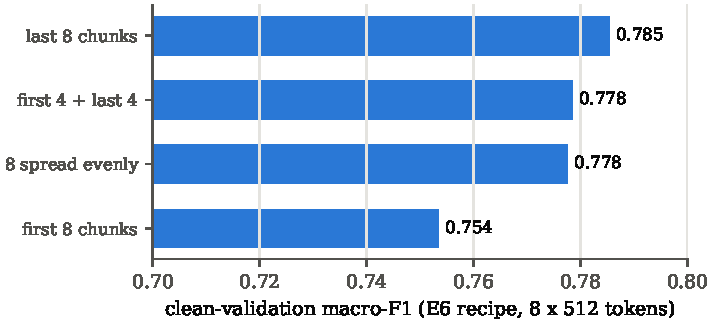
\includegraphics[width=0.7\linewidth]{figs/ablation.pdf}
\caption{Section ablation: E6 recipe with different chunk selections (same 8 $\times$ 512 tokens).}
\label{fig:ablation}\end{figure}

\subsection{Knowledge distillation and efficiency}
\begin{table}[H]\centering\small
\caption{Size, compute and memory.  Test inference = seconds to score the \ntest{} test documents.}\label{tab:eff}
\resizebox{\linewidth}{!}{\begin{tabular}{lllrrrrrr}\toprule
Run & Arch & Method & Total & Trainable & Train (min) & Test infer. (s) & Peak GB & Ckpt MB\\\midrule
\tabinput{tables/efficiency.tex}
\bottomrule\end{tabular}}\end{table}
The KD student (E8) has \kdparams{} parameters against \teacherparams{} for its teacher E6 and keeps
\kdretain\% of the teacher's validation macro-F1; test inference takes \kdinfer{} s against \teacherinfer{} s.

\subsection{Ensembles}
\begin{table}[H]\centering\small
\caption{Probability-averaging ensembles (threshold tuned on the averaged validation probabilities).}\label{tab:ens}
\begin{tabular}{llrrrr}\toprule
Name & Members & F1 & thr & P & R\\\midrule
\tabinput{tables/ensembles.tex}
\bottomrule\end{tabular}\end{table}

\subsection{Errors of the best single model}
E6 makes \nfp{} false positives (predicted allowed, actually dismissed) and \nfn{} false negatives on the
validation set.

\begin{figure}[H]\centering
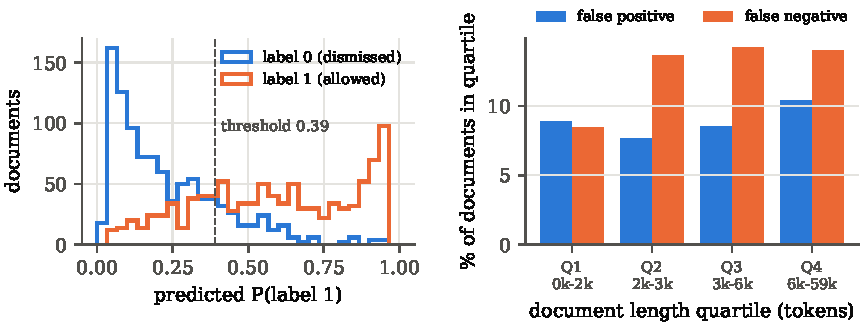
\includegraphics[width=0.95\linewidth]{figs/errors.pdf}
\caption{E6 on clean validation. Left: predicted probability of label 1 per true class. Right: false-positive
and false-negative rate by document-length quartile.}
\label{fig:errors}\end{figure}

\begin{table}[H]\centering\small
\caption{E6 by document-length quartile (tokens).}\label{tab:errlen}
\begin{tabular}{llrrrr}\toprule
Quartile & Length & Docs & Macro-F1 & FP & FN\\\midrule
\tabinput{tables/errors_len.tex}
\bottomrule\end{tabular}\end{table}

\subsection{Submission files}
\nzips{} format-checked zips are in \code{p4/submissions/} (an experiment with two zips has identical
predictions in both).
\authorbox{leaderboard scores}{Add the Codabench test macro-F1, precision and recall of each uploaded submission
and say which six or more count towards the requirement.}
{\scriptsize\begin{longtable}{l}\toprule File\\\midrule\endhead
\tabinput{tables/submissions.tex}
\bottomrule\end{longtable}}

% =====================================================================
\section{Analysis}
\authorbox{analysis of the results}{The course rules do not allow LLM-written result analysis.  Questions the
course asks (§10.5), with the evidence above:
\begin{itemize}
  \item Which adaptation techniques are effective, and can parameter-efficient methods retain full fine-tuning
  performance (\autoref{tab:results}, \autoref{fig:params})?
  \item How do long-document representations and chunk selection affect prediction (\autoref{fig:ablation})?
  \item Which sections are useful, based on the ablation?
  \item How does class imbalance affect performance (\autoref{fig:thr})?
  \item What characterises false positives and false negatives (\autoref{fig:errors}, \autoref{tab:errlen})?
  \item Does distillation keep performance while reducing size and compute (\autoref{tab:eff})?
  \item How well does the Phase-1 model transfer to CJPE?
\end{itemize}}

\section{Limitations and next steps}
Facts that limit the conclusions (the interpretation is the author's):
\begin{itemize}
  \item One seed per run; the validation set has \nval{} documents and the threshold is tuned on it, so the
  reported F1 is slightly optimistic.
  \item Eight chunks cover the whole document for only \shortereight\% of validation documents.
  \item AdaLoRA (E5) and BitFit (E4) were run with one setting each.
  \item The PEFT learning rate was changed once during the phase (\autoref{sec:train}).
  \item The provided test labels and the test/dev overlap (\autoref{sec:data}) mean the public leaderboard may
  not reflect held-out performance for every participant.
\end{itemize}
\authorbox{what you would do next}{With more time or compute: \ldots}

\section{Conclusions}
\authorbox{conclusions}{Summarise what you conclude from the experiments, in your own words.}

\section{Reproducibility}
\noindent{\small\begin{tabularx}{\linewidth}{l>{\raggedright\arraybackslash}X}
Token cache & built on first use by \code{cj/data.py} (\code{build\_cache})\\
Experiments E1--E7 + zips & \code{bash run\_all.sh}\\
One experiment & \code{python train.py --config configs/e6\_a4\_partial.yaml}\\
Teacher logits + KD & \code{python dump\_logits.py --run runs/E6\_a4\_partial}; \code{bash run\_all.sh configs/e8\_kd\_a4\_small.yaml}\\
Section ablation & \code{bash run\_all.sh configs/a\_e6\_first.yaml configs/a\_e6\_first\_last.yaml configs/a\_e6\_spread.yaml}\\
Ensemble zip & \code{python make\_submission.py --run runs/E6\_a4\_partial runs/E7\_a3\_gradual ... --name ENS\_top5}\\
Figures and tables & \code{python p4/report/make\_figures.py}\\
\end{tabularx}}
\authorbox{repository link}{GitHub: \url{https://github.com/...}}

\section*{LLM declaration}
\authorbox{LLM declaration (mandatory)}{Fill in the course questionnaire.  Describe honestly which parts used
an LLM assistant (for example the data pipeline, model and training code, figures and this report's
methods/results text) and which parts are your own (design decisions, hyperparameters, analysis, conclusions).}

\begin{thebibliography}{99}\small
\bibitem{benzaken2022bitfit} E.~Ben Zaken, S.~Ravfogel, Y.~Goldberg. BitFit: Simple parameter-efficient fine-tuning for transformer-based masked language-models. ACL 2022.
\bibitem{bihany2025lorma} H.~Bihany, S.~Patel, A.~Modi. LoRMA: Low-rank multiplicative adaptation for LLMs. Findings of ACL 2025.
\bibitem{cho2014gru} K.~Cho et al. Learning phrase representations using RNN encoder--decoder for statistical machine translation. EMNLP 2014.
\bibitem{hinton2015kd} G.~Hinton, O.~Vinyals, J.~Dean. Distilling the knowledge in a neural network. arXiv:1503.02531, 2015.
\bibitem{houlsby2019adapters} N.~Houlsby et al. Parameter-efficient transfer learning for NLP. ICML 2019.
\bibitem{howard2018ulmfit} J.~Howard, S.~Ruder. Universal language model fine-tuning for text classification. ACL 2018.
\bibitem{malik2021ildc} V.~Malik et al. ILDC for CJPE: Indian legal documents corpus for court judgment prediction and explanation. ACL 2021.
\bibitem{yang2016han} Z.~Yang et al. Hierarchical attention networks for document classification. NAACL 2016.
\bibitem{zhang2023adalora} Q.~Zhang et al. AdaLoRA: Adaptive budget allocation for parameter-efficient fine-tuning. ICLR 2023.
\end{thebibliography}
\end{document}
